\documentclass[conference]{IEEEtran}

\usepackage{cite}
\usepackage{amsmath,amssymb,amsfonts}
\usepackage{graphicx}
\usepackage{textcomp}
\usepackage{xcolor}
\usepackage{booktabs}
\usepackage{multirow}
\usepackage{url}

% Numbers in tables are generated by make_paper_tables.py from results/*.csv;
% numbers in the text are traced to their source files in paper_notes/number_audit.md.

\title{Where Refinement Goes and What It Costs: A Controlled Study of Marking Strategies for Adaptive Mesh Refinement on Viscous Burgers' Equation}

\author{
\IEEEauthorblockN{Achyuta Rag}
\IEEEauthorblockA{
\textcolor{red}{[Department]}, University of California, Irvine\\
Irvine, CA, USA\\
achyutr@uci.edu
}
}

\begin{document}

\maketitle

\begin{abstract}
Adaptive mesh refinement (AMR) involves two distinct decisions: where to refine, set by an error indicator and a marking rule, and how the solution improves once a cell is refined, set by the numerical scheme. We compare three marking rules (a relative threshold, deterministic top-$K$ selection, and temperature-scaled Gumbel top-$K$ sampling) on the one-dimensional viscous Burgers' equation, with budgets matched by final cell count and cost also measured as total cell updates. In controlled experiments we vary scheme order, refinement timing, the coarsening threshold, and the error indicator. The marking rules differ in final error by 3--30\%, and Gumbel sampling shows no consistent advantage over deterministic top-$K$ selection in accuracy or mesh stability. Scheme order changes AMR error 5.7--7.0-fold; the indicator and refinement timing change it by up to 1.85-fold and 1.59-fold respectively. With a first-order scheme, uniform refinement is more accurate than AMR at matched work in every configuration tested; with a second-order scheme and a gradient indicator, AMR is ahead only at small budgets. A curvature indicator reduces error by 12--46\% at matched cell count and is the only configuration in which AMR beats uniform refinement at matched work at every budget tested, with uniform error 1.05--1.43 times the AMR error against actual uniform runs given at least as much work. Evaluations of marking strategies should therefore control scheme order, indicator, refinement timing, and the cost measure.
\end{abstract}

\begin{IEEEkeywords}
Adaptive mesh refinement, marking strategies, error indicators, finite volume methods, Burgers' equation, numerical diffusion
\end{IEEEkeywords}

\section{Introduction}

Adaptive mesh refinement concentrates resolution where a numerical solution is hard to approximate. Each cycle of an adaptive method can be summarized as \emph{solve, estimate, mark, refine}: an indicator assigns each cell a score, a marking rule turns the scores into a set of cells to refine, and the mesh is then refined and coarsened \cite{berger1984,berger1989}. Two different questions are bundled in this loop. The first is \emph{where} refinement is needed, which the indicator and marking rule decide. The second is \emph{how} the approximation improves after a cell is refined, which the numerical scheme, the transfer of data to new cells, and the time step decide.

This paper studies the first question by comparing marking rules, and shows that the answer depends on the second. We compare three rules on a scalar conservation law with a steepening front: a relative threshold rule, deterministic top-$K$ selection, and a stochastic rule that samples $K$ cells without replacement with probabilities given by a temperature-scaled softmax of the indicator, implemented with the Gumbel-top-$k$ trick \cite{kool2019}. The stochastic rule was the original object of this study. The question was whether smoothing the marking decision changes accuracy or mesh stability at a fixed budget.

Answering that question requires that the comparison not be dominated by other factors. We identify and test four: the numerical diffusion of the scheme, the time at which refinement is first allowed, the indicator used to rank cells, and the measure of cost against which accuracy is compared.

The contributions are:
\begin{itemize}
\item a budget-matched comparison of three marking rules, with cost measured both as final cell count and as total cell updates, for first- and second-order schemes;
\item a control experiment that separates the effect of resolution near the forming front from resolution elsewhere during the period before refinement starts;
\item ablations of the coarsening threshold and of the indicator (gradient versus curvature), reporting accuracy together with its computational cost;
\item a work-matched comparison against uniform refinement that uses actual uniform runs bracketing each AMR budget rather than interpolation alone.
\end{itemize}

Section~\ref{sec:related} reviews related work, Section~\ref{sec:methods} describes the problem, discretization, and experimental protocol, Section~\ref{sec:results} reports the results, and Sections~\ref{sec:discussion}--\ref{sec:conclusion} discuss them, state limitations, and conclude.

\section{Related Work}
\label{sec:related}

Block-structured AMR for hyperbolic problems was introduced by Berger and Oliger \cite{berger1984} and extended to shock hydrodynamics with conservative interface treatment by Berger and Colella \cite{berger1989}. Both use local time stepping (subcycling), so finer levels take smaller steps without forcing small steps on coarse cells. Our solver does not subcycle, and Section~\ref{sec:results} shows how this affects cost.

For adaptive finite element methods, marking rules have been studied theoretically. The maximum strategy of Babu\v{s}ka and Rheinboldt \cite{babuska1978} refines cells whose indicator exceeds a fraction of the largest indicator. Our threshold rule is of this type. D\"orfler's bulk criterion \cite{dorfler1996} marks a minimal set of cells that carries a fixed fraction of the total estimated error, and is central to convergence and optimality theory for adaptive methods \cite{carstensen2014}. We do not test D\"orfler marking here; it is the natural next baseline.

Indicators based on second differences, normalized to be scale-independent, were proposed by L\"ohner \cite{lohner1987} and are widely used for unstructured adaptive computations. The curvature indicator used in our ablation is a simpler, unnormalized relative of that idea.

The finite volume schemes we use are standard: the local Lax--Friedrichs (Rusanov) flux \cite{rusanov1962}, slope-limited MUSCL reconstruction \cite{vanleer1979}, and strong-stability-preserving Runge--Kutta time stepping \cite{gottlieb2001}. Conservation form is required for correct shock speeds \cite{leveque2002}.

Stochastic marking appears implicitly in reinforcement-learning approaches to AMR, where a learned policy selects cells to refine \cite{yang2023}. The Gumbel-top-$k$ trick \cite{kool2019} gives an exact way to sample $k$ items without replacement from a softmax distribution, and a temperature parameter interpolates between deterministic top-$k$ selection and uniform sampling. We use it as a simple, untrained stochastic marker.

This paper does not propose a new adaptive method. It asks how much the marking rule matters once the other parts of the adaptive loop are controlled.

\section{Materials and Methods}
\label{sec:methods}

\subsection{Test Problem}

We solve the viscous Burgers' equation
\begin{equation}
u_t + \left(\tfrac{1}{2}u^2\right)_x = \nu\, u_{xx}, \qquad x \in [0,1),\; t \in (0, T],
\label{eq:burgers}
\end{equation}
with periodic boundary conditions, $\nu = 0.01$, $T = 0.3$, and initial data $u(x,0) = \sin(2\pi x) + 0.5$. The solution steepens into a front located near $x = 0.65$ at $t = T$ (Fig.~\ref{fig:solution}). With $\nu = 0.01$ the front is a resolved viscous layer rather than a discontinuity.

\subsection{Discretization}

To discretize~\eqref{eq:burgers}, the domain is divided into cells $I_i$ of width $h_i$, and the cell averages $u_i$ are advanced in conservation form
\begin{equation}
\frac{du_i}{dt} = -\frac{F_{i+1/2} - F_{i-1/2}}{h_i}, \qquad
F_{i+1/2} = \hat f\!\left(u^-_{i+1/2}, u^+_{i+1/2}\right) - \nu\,\frac{u_{i+1}-u_i}{\bar h_{i+1/2}},
\label{eq:fv}
\end{equation}
where $\bar h_{i+1/2}$ is the distance between cell centers and $\hat f$ is the Rusanov flux
\begin{equation}
\hat f(a,b) = \tfrac{1}{4}\left(a^2 + b^2\right) - \tfrac{1}{2}\max(|a|,|b|)\,(b - a).
\label{eq:rusanov}
\end{equation}
Both schemes below use~\eqref{eq:fv} with the flux~\eqref{eq:rusanov} and differ only in the face states and the time integrator. The \emph{first-order} scheme uses the cell averages as face states ($u^-_{i+1/2} = u_i$, $u^+_{i+1/2} = u_{i+1}$) with forward Euler time stepping. Its numerical viscosity is approximately $\tfrac{1}{2}|u|h$, about $0.02$ on cells of width $1/32$ where $|u| \approx 1.25$, roughly twice the physical viscosity. The \emph{second-order} scheme reconstructs face states from minmod-limited slopes computed with center-to-center spacings on the non-uniform mesh \cite{vanleer1979}, and uses the two-stage SSP Runge--Kutta method \cite{gottlieb2001}. Both schemes use a single global time step
\begin{equation}
\Delta t = 0.4\,\min\!\left(\frac{h_{\min}}{\max_i |u_i|},\; \frac{h_{\min}^2}{2\nu}\right),
\label{eq:dt}
\end{equation}
set by the smallest cell $h_{\min}$; there is no subcycling.

\subsection{Mesh and Refinement Operations}

The mesh is dyadic. A base mesh of 32 cells may be refined by up to three levels (smallest width $1/256$) in the main experiments, and up to five levels ($1/1024$) in one ablation. Refinement splits a cell into two halves. With the first-order scheme both children receive the parent value. With the second-order scheme they receive $u_i \mp \tfrac{1}{4} h_i s_i$, where $s_i$ is the minmod slope. Both choices conserve the cell integral exactly. Coarsening merges only two cells that share a parent, never produces cells wider than the base mesh, and assigns the width-weighted average. Regridding is attempted at $20$ equally spaced times in $(0, T]$, so all methods have the same opportunities to regrid regardless of their time step.

\subsection{Indicators, Gate, and Marking Rules}

Two indicators are used: the \emph{gradient} indicator $\eta^{\nabla}_i = h_i\,|\partial_x u|_i$, and, in the indicator ablation, the \emph{curvature} indicator $\eta^{\kappa}_i = h_i^2\,|\partial_{xx} u|_i$, with the standard three-point second difference on the non-uniform mesh. The curvature indicator vanishes on linear profiles.

Refinement is \emph{gated}: a regrid is carried out only if $\max_i \eta^{\nabla}_i / \operatorname{median}_i \eta^{\nabla}_i \ge 3.5$, which prevents refinement during the smooth early transient. With the base mesh this gate first opens at $t_g = 0.105$.

Given indicator values $\eta_i$, the three marking rules are:
\begin{itemize}
\item \emph{Threshold}: refine cells with $\eta_i > \theta \max_j \eta_j$. This is a maximum strategy \cite{babuska1978}. Earlier versions of this work called it a hysteresis marker; it keeps no state between regrid events.
\item \emph{Top-$K$}: refine the $K$ cells with the largest $\eta_i$ among cells that are not already at the finest level.
\item \emph{Gumbel top-$K$}: with $\tilde\eta_i = \eta_i / \max_j \eta_j$, refine the $K$ eligible cells with the largest $\tilde\eta_i / \tau + g_i$, where the $g_i$ are independent standard Gumbel samples \cite{kool2019}. This samples $K$ cells without replacement from $\operatorname{softmax}(\tilde\eta/\tau)$. We use $\tau = 0.1$. Normalizing by the maximum makes $\tau$ independent of the scale of $\eta$.
\end{itemize}
All rules share one coarsening rule: a sibling pair is merged if both cells have $\eta_i < 0.05 \max_j \eta_j$ after refinement.

\subsection{Error, Cost, and Stability Measures}

Errors are $L^2$ norms against a uniform 4096-cell solution computed with the same scheme. Comparing 4096 with 8192 cells gives reference errors of $4.4\times10^{-4}$ (first order) and $4.0\times10^{-6}$ (second order), below every error reported here. The AMR solution is interpolated linearly from cell centers to the reference cell centers. The error is also split into a \emph{shock window}, $|x - x_f| < 0.05$ around the final front location $x_f$, and the remaining \emph{smooth region}.

Cost is reported in two ways: the \emph{final cell count}, and the \emph{work}, defined as the total number of cell updates (the sum over time steps of the number of cells). Because the time step~\eqref{eq:dt} is global, work grows with both the number of cells and the depth of refinement.

\emph{Grid turnover} is the Jaccard distance between the sets of positions covered by finest-level cells at consecutive regrid events, measured on 2048 fixed reference points. It is computed only for pairs of events in which both sets are non-empty. We report the mean over valid pairs together with the number of pairs, and treat turnover as undefined for runs with none.

\subsection{Experimental Protocol}

For each target final cell count, each marking rule's budget parameter ($\theta$ or $K$) is chosen by a grid search so that its final cell count is closest to the target. The deterministic rules are run once. Gumbel top-$K$ is run with 20 seeds in the main comparison and 10 seeds in the ablations, and we report mean and standard deviation. Uniform grids are run at the same targets and, for the work-matched comparison, at every $n = 32, 36, \ldots, 320$.

Before the experiments, the implementation was checked as follows. The first-order scheme reproduces the original solver to $4\times10^{-16}$. On smooth data at $t = 0.05$, the observed orders of accuracy are $0.80$--$1.03$ (first order) and $1.98$--$2.02$ (second order) on uniform grids, and $0.91$--$1.07$ and $1.79$--$2.04$ on grids with a refined patch. Total mass is conserved to within $4.4\times10^{-16}$ in every adaptive run. Top-$K$ refines exactly $\min(K, \text{eligible})$ cells at every event, and the mesh remains dyadic with all cells no wider than the base mesh.

All code, the CSV files behind every table and figure, and scripts that regenerate them are available from the author \textcolor{red}{[add repository link]}.

\section{Results}
\label{sec:results}

\subsection{Budget-Matched Comparison and Scheme Order}

Table~\ref{tab:sweep} and Fig.~\ref{fig:cost} compare the three marking rules and uniform refinement. With the second-order scheme, the three rules give errors within 3\% of each other at about 64 cells, and within 15\% at about 192 cells. At about 128 cells, the Gumbel top-$K$ error is 30\% higher than the threshold error, part of which reflects a residual budget difference (112 versus 126 final cells). Gumbel and deterministic top-$K$ show no consistent difference: Gumbel is less accurate at about 128 cells and more accurate at about 192, by about two and one seed standard deviations respectively.

Scheme order matters much more. At matched budgets, the second-order scheme reduces AMR error by a factor of 5.7--7.0. It also changes the comparison with uniform refinement. Per final cell, second-order AMR is 2.7 times more accurate than a uniform 64-cell grid, comparable to a uniform 128-cell grid, and less accurate than a uniform 192-cell grid. First-order AMR is more accurate per cell only below about 96 cells. Measured by work (Fig.~\ref{fig:cost}, right), the picture changes again. With the first-order scheme, uniform refinement is more accurate than AMR at matched work in all 21 configurations, for every marking rule and budget: the AMR error is 1.3--1.6 times the uniform error. With the second-order scheme, AMR with the gradient indicator is ahead only at small budgets (Section~\ref{sec:workmatched}).

\begin{table*}[t]
\caption{Budget-matched comparison ($\nu = 0.01$, three refinement levels, gradient indicator). Gumbel top-$K$: mean $\pm$ standard deviation over 20 seeds. Work is total cell updates. Turnover: mean Jaccard turnover (number of valid event pairs).}
\label{tab:sweep}
\centering
\begin{tabular}{llrrrr}
\toprule
Target & Method & Cells & $L^2$ error ($\times10^{-3}$) & Work ($\times10^{3}$) & Turnover \\
\midrule
\multicolumn{6}{l}{\emph{Second-order scheme (MUSCL, SSP-RK2)}} \\
64 & Threshold & 53 & 7.47 & 16.6 & 0.21 (4) \\
 & Top-$K$ & 65 & 7.25 & 19.2 & 0.23 (5) \\
 & Gumbel top-$K$ & 68 & 7.44 $\pm$ 0.54 & 23.4 & 0.25 (6) \\
 & Uniform & 64 & 19.94 & 4.4 & -- \\
\addlinespace
128 & Threshold & 126 & 4.73 & 65.9 & 0.11 (10) \\
 & Top-$K$ & 130 & 5.39 & 41.8 & 0.16 (7) \\
 & Gumbel top-$K$ & 112 & 6.14 $\pm$ 0.33 & 35.4 & 0.22 (7) \\
 & Uniform & 128 & 5.98 & 31.5 & -- \\
\addlinespace
192 & Threshold & 196 & 4.42 & 109.8 & 0.10 (11) \\
 & Top-$K$ & 195 & 5.07 & 61.2 & 0.32 (7) \\
 & Gumbel top-$K$ & 195 & 4.74 $\pm$ 0.29 & 64.8 & 0.28 (8) \\
 & Uniform & 192 & 2.80 & 106.2 & -- \\
\addlinespace
\multicolumn{6}{l}{\emph{First-order scheme (Rusanov, forward Euler)}} \\
64 & Threshold & 56 & 42.80 & 18.9 & 0.24 (3) \\
 & Top-$K$ & 64 & 42.93 & 15.4 & 0.29 (2) \\
 & Gumbel top-$K$ & 62 & 43.96 $\pm$ 0.80 & 19.5 & 0.30 (4) \\
 & Uniform & 64 & 51.25 & 4.4 & -- \\
\addlinespace
128 & Threshold & 129 & 31.57 & 60.9 & 0.10 (9) \\
 & Top-$K$ & 125 & 37.06 & 38.2 & 0.19 (5) \\
 & Gumbel top-$K$ & 137 & 36.23 $\pm$ 0.55 & 40.0 & 0.25 (6) \\
 & Uniform & 128 & 26.57 & 31.5 & -- \\
\addlinespace
192 & Threshold & 193 & 28.78 & 102.5 & 0.09 (10) \\
 & Top-$K$ & 180 & 32.49 & 53.3 & 0.37 (5) \\
 & Gumbel top-$K$ & 189 & 33.14 $\pm$ 0.58 & 56.9 & 0.27 (7) \\
 & Uniform & 192 & 17.72 & 106.2 & -- \\
\bottomrule
\end{tabular}

\end{table*}

\begin{figure*}[t]
\centering
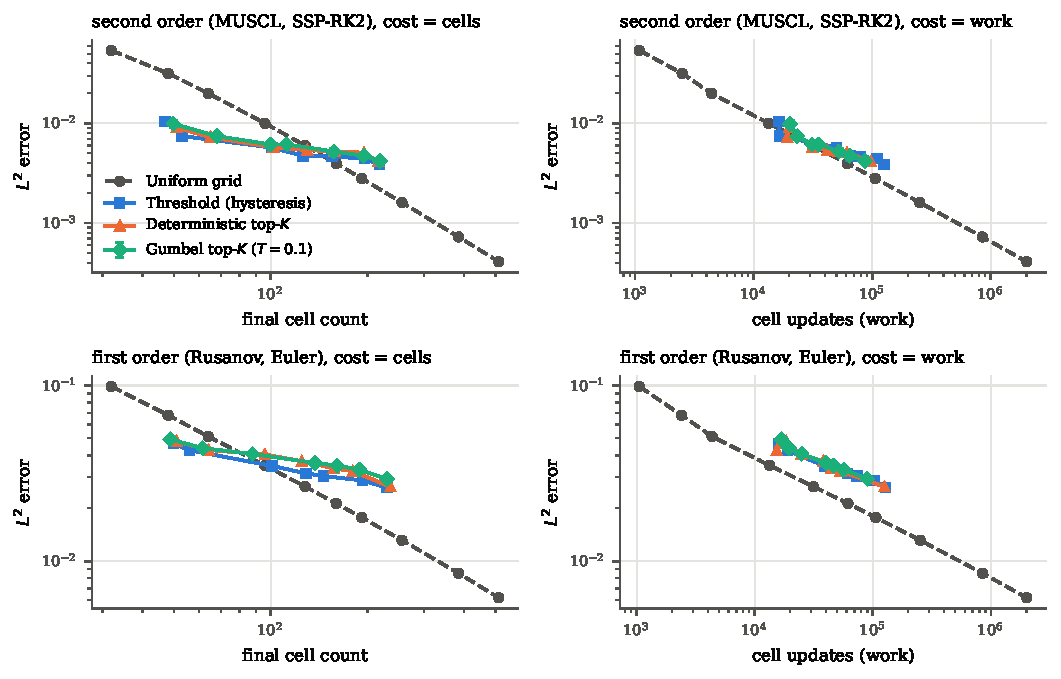
\includegraphics[width=\textwidth]{figures/fig4_error_vs_cost.pdf}
\caption{$L^2$ error against final cell count (left) and work (right) for the second-order (top) and first-order (bottom) schemes, gradient indicator. Gumbel top-$K$ error bars show one standard deviation over 20 seeds.}
\label{fig:cost}
\end{figure*}

\subsection{Refinement Timing}

The gate delays all refinement until $t_g = 0.105$. To test whether the resolution available before $t_g$ matters, and where, we ran four variants that differ \emph{only} on $[0, t_g]$: the base mesh (A, identical to the gated run), finest-level resolution everywhere (C), finest-level resolution on $[0.375, 0.75]$, which contains the forming front throughout this period (D), and finest-level resolution on a region of the same width away from the front (E). At $t_g$ each solution is averaged conservatively onto the base mesh and all variants then run the same gated AMR to $T$.

Table~\ref{tab:timing} and Fig.~\ref{fig:timing} show the results for the second-order scheme at about 128 final cells. Resolving the forming front recovers 61--82\% of the difference in final error between A and C, while the same resolution away from the front recovers 16--24\%. The error carried into the AMR phase shows the same pattern. With the first-order scheme, neither region alone recovered more than about 30\% of the difference, consistent with numerical diffusion acting throughout the domain. Removing the gate altogether also lowers the error, but the ungated runs end with 182--213 cells instead of about 128, so that comparison is not budget-matched.

\begin{table}[t]
\caption{Early-phase control, second-order scheme, about 128 final cells. Error at $t_g$ is measured on the base mesh. Brackets: share of the A--C difference in final error that the arm recovers. Gumbel: mean of 10 seeds.}
\label{tab:timing}
\centering
\resizebox{\columnwidth}{!}{\begin{tabular}{lrrrr}
\toprule
Early-phase mesh & Error at $t_g$ & Threshold & Top-$K$ & Gumbel \\
 & ($\times10^{-3}$) & \multicolumn{3}{c}{final $L^2$ error ($\times10^{-3}$) [gap recovered]} \\
\midrule
A: base mesh (gated) & 11.83 & 4.73 & 5.39 & 6.22 \\
E: fine away from front & 11.11 & 4.39 [24\%] & 5.08 [16\%] & 5.78 [22\%] \\
D: fine around front & 4.42 & 3.56 [82\%] & 4.18 [61\%] & 4.88 [67\%] \\
C: fine everywhere & 0.21 & 3.31 & 3.40 & 4.22 \\
\bottomrule
\end{tabular}
}
\end{table}

\begin{figure}[t]
\centering
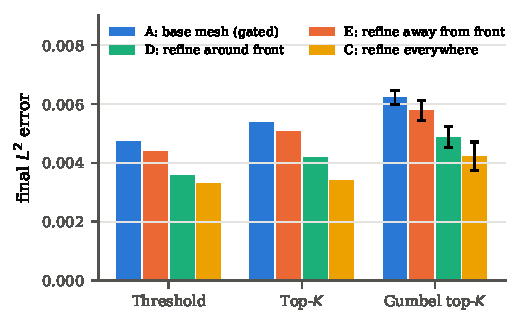
\includegraphics[width=\columnwidth]{figures/fig6_timing_control.pdf}
\caption{Final $L^2$ error for the four early-phase meshes (Table~\ref{tab:timing}). Error bars: one standard deviation over 10 seeds (Gumbel top-$K$).}
\label{fig:timing}
\end{figure}

\subsection{Where Refinement Goes}

The final meshes (Fig.~\ref{fig:meshes}) show that refinement with the gradient indicator is not concentrated at the front. At about 128 cells, 103 of 126 cells (threshold) and 107 of 130 cells (top-$K$) lie outside the shock window and are finer than the base mesh. The cause is visible in Fig.~\ref{fig:solution}: on the smooth ramp the gradient indicator is a sizeable fraction of its maximum. When the gate opens, the ramp's indicator is 23--25\% of the maximum on uniform grids of 32--256 cells, so the first regrid events refine much of the domain. At $T$ the median indicator in the smooth region of the final mesh is still about 11\% of the maximum, above the 5\% coarsening threshold, so these cells are never coarsened.

Raising the coarsening threshold does not fix this. With thresholds of 0.10, 0.15, and 0.20, the largest final mesh reached in any run shrinks to 124, 96, and 89 cells, so the coarsening rule rather than the marking rule sets the budget. The share of cells in the shock window at comparable cell counts is essentially unchanged (0.28 at 78 cells with threshold 0.15, against 0.22--0.34 at 65--102 cells with threshold 0.05). At large $K$, cells refined at one event are merged at the next, with up to 602--677 merges per run. Accuracy at matched cell count does not improve.

\begin{figure}[t]
\centering
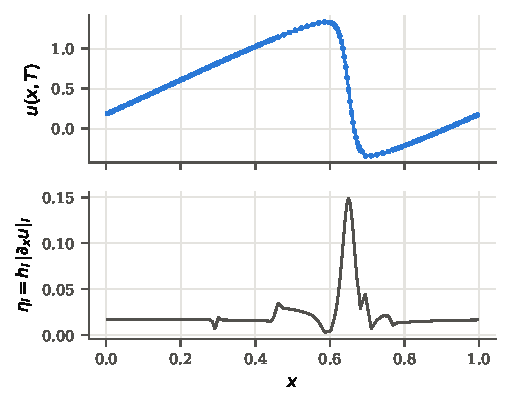
\includegraphics[width=\columnwidth]{figures/fig1_solution_indicator.pdf}
\caption{Solution at $t = T$ (top) and gradient indicator (bottom), threshold marking, second-order scheme, 126 cells.}
\label{fig:solution}
\end{figure}

\begin{figure}[t]
\centering
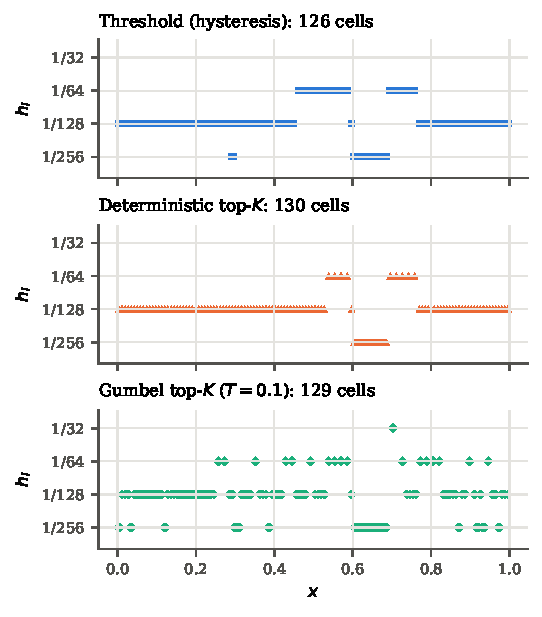
\includegraphics[width=\columnwidth]{figures/fig3_final_meshes.pdf}
\caption{Final cell widths for the three marking rules at about 128 cells (second-order scheme, gradient indicator, Gumbel seed 0).}
\label{fig:meshes}
\end{figure}

\subsection{Indicator Ablation and Its Cost}

We compare the gradient and curvature indicators while holding the gradient-based contrast gate fixed. The comparison therefore isolates the effect of the marking indicator conditional on the same refinement-activation mechanism. It is not a comparison of two complete, independently designed AMR strategies. The gate is held fixed because refinement timing strongly affects final error (Table~\ref{tab:timing}); a curvature-based gate would open at a different time, and the resulting difference could not be attributed to the indicator. The gate opens at $t_g = 0.105$ in both arms. It is then re-evaluated at each regrid time on each arm's own mesh, so the later regrid schedules differ. For top-$K$ at about 64 cells, for example, the gradient arm regridded at 8 of the 14 scheduled times from $t_g$ to $T$ and the curvature arm at 4 (Table~\ref{tab:indicator}, which reports the number of regrid events for every configuration).

With three levels (Table~\ref{tab:indicator}), the curvature indicator reduces error by 12--46\% at matched final cell count, for every marking rule and budget. At about 80 cells it also roughly halves the number of refined cells outside the shock window (29--38 against 56--60); at smaller budgets these counts are small and the change is mixed. Its cost depends on the budget. At about 48 cells it uses less work than the gradient indicator, at about 64 cells 1.0--1.6 times as much, and at about 80 cells 1.8--2.7 times as much: the target exceeds what the front can absorb at the finest level, so cells refined at one event are merged at the next (228--378 refinements and 182--330 merges per run, against 56--63 and 8--9 for the gradient indicator). The time-averaged cell count (89--107) then exceeds the final count (75--80).

\begin{table*}[t]
\caption{Gradient versus curvature indicator, second-order scheme, three refinement levels, shared gradient-based gate. Steps: time steps taken. Refined/merged: totals per run. Regrids: events at which the gate was open. Turnover: mean (number of valid event pairs). Gumbel top-$K$: mean $\pm$ standard deviation over 10 seeds.}
\label{tab:indicator}
\centering
\resizebox{\textwidth}{!}{\begin{tabular}{llrrrrrrr}
\toprule
Target & Indicator / method & Cells & $L^2$ ($\times10^{-3}$) & Work ($\times10^{3}$) & Steps & Refined/merged & Regrids & Turnover \\
\midrule
48 & gradient, Threshold & 47 & 10.49 & 16.4 & 387 & 18/3 & 10.0 & 0.25 (5) \\
 & gradient, Top-$K$ & 51 & 9.08 & 19.9 & 461 & 22/3 & 11.0 & 0.25 (7) \\
 & gradient, Gumbel top-$K$ & 50 & 10.06 $\pm$ 0.86 & 20.7 & 468 & 24/6 & 11.9 & 0.26 (8) \\
 & curvature, Threshold & 50 & 6.45 & 15.5 & 304 & 26/8 & 9.0 & 0.25 (2) \\
 & curvature, Top-$K$ & 51 & 7.66 & 15.9 & 350 & 22/3 & 11.0 & 0.33 (4) \\
 & curvature, Gumbel top-$K$ & 49 & 8.88 $\pm$ 0.70 & 13.6 & 305 & 21/4 & 10.5 & 0.44 (3) \\
\addlinespace
64 & gradient, Threshold & 53 & 7.47 & 16.6 & 341 & 28/7 & 7.0 & 0.21 (4) \\
 & gradient, Top-$K$ & 65 & 7.25 & 19.2 & 378 & 40/7 & 8.0 & 0.23 (5) \\
 & gradient, Gumbel top-$K$ & 70 & 7.56 $\pm$ 0.58 & 23.1 & 431 & 45/8 & 9.0 & 0.23 (6) \\
 & curvature, Threshold & 64 & 4.60 & 26.6 & 415 & 42/10 & 4.0 & 0.38 (1) \\
 & curvature, Top-$K$ & 63 & 5.33 & 19.5 & 341 & 36/5 & 4.0 & 0.46 (1) \\
 & curvature, Gumbel top-$K$ & 58 & 5.32 $\pm$ 0.57 & 26.1 & 461 & 41/15 & 5.9 & 0.51 (3) \\
\addlinespace
80 & gradient, Threshold & 80 & 6.57 & 26.0 & 378 & 57/9 & 9.0 & 0.18 (6) \\
 & gradient, Top-$K$ & 80 & 6.29 & 22.5 & 387 & 56/8 & 7.0 & 0.26 (4) \\
 & gradient, Gumbel top-$K$ & 87 & 6.69 $\pm$ 0.57 & 25.4 & 409 & 63/8 & 9.0 & 0.20 (6) \\
 & curvature, Threshold & 75 & 3.55 & 61.9 & 581 & 263/220 & 14.0 & 0.34 (11) \\
 & curvature, Top-$K$ & 80 & 3.55 & 60.4 & 581 & 378/330 & 14.0 & 0.37 (11) \\
 & curvature, Gumbel top-$K$ & 79 & 3.78 $\pm$ 0.08 & 47.2 & 532 & 229/182 & 12.7 & 0.25 (10) \\
\bottomrule
\end{tabular}
}
\end{table*}

\paragraph*{Depth and the global time step}
For $\nu = 0.01$ and $\max|u| \approx 1.35$, the diffusive limit in~\eqref{eq:dt} is the smaller one whenever $h_{\min} < 2\nu/\max|u| \approx 1/68$. On every refined level, therefore, $\Delta t \propto h_{\min}^2$, and each additional level multiplies the number of time steps by up to four. With three levels the AMR runs took 300--580 steps. With five levels, runs that reached $h_{\min} = 1/1024$ took 1519--4526 steps, against 984 for a uniform 256-cell grid. Deeper refinement thus raises the cost of every cell in the mesh. Five-level runs reached their lowest errors at about 94--110 cells with the curvature indicator ($3.0\times10^{-3}$ for top-$K$), but at a work of about $3\times10^{5}$ cell updates.

\subsection{Work-Matched Comparison with Uniform Refinement}
\label{sec:workmatched}

Because uniform grids were run at every $n = 32, 36, \ldots, 320$, each AMR configuration's mean work lies between two actual uniform runs whose work differs by 4--13\%. Table~\ref{tab:work} reports both neighbours and the ratio of uniform to AMR error at the AMR work, using log-log interpolation between the neighbours and a conservative rule that compares against the neighbour with \emph{more} work than the AMR run. Linear interpolation and the nearest neighbour give ratios within 8\% of these; all four values are in the accompanying data. We claim an AMR advantage only where the conservative ratio exceeds one.

With the curvature indicator and three levels, AMR is more accurate than uniform refinement at matched work in every configuration, by factors of 1.05--1.43 under the conservative rule. For Gumbel top-$K$, 70\% of seeds beat uniform refinement at about 48 cells, and all seeds do at about 64 and 80 cells. With the gradient indicator, the conservative ratio ranges from 0.76 to 1.16. AMR is ahead only at about 64 cells (threshold 1.16, top-$K$ 1.05), at about 80 cells for top-$K$ (1.14) and, marginally, Gumbel top-$K$ (1.01, with 50\% of seeds ahead), and at about 96 cells for top-$K$ (1.04); uniform refinement is more accurate in the main sweep at all budgets of 128 cells or more (0.61--0.89). With five levels, uniform refinement is more accurate at matched work in every configuration, for both indicators (conservative ratios 0.21--0.83), because of the time-step penalty above.

\begin{table*}[t]
\caption{Work-matched comparison with uniform refinement (second-order scheme, three levels). Uniform below/above: the actual uniform runs whose work brackets the AMR work. Errors in units of $10^{-3}$. Ratio: uniform error divided by AMR error, by log-log interpolation and by the conservative rule (uniform run with more work); a value above one favours AMR. Gumbel top-$K$: brackets give the share of seeds more accurate than uniform at their own work.}
\label{tab:work}
\centering
\resizebox{\textwidth}{!}{\begin{tabular}{llrrrrrrr}
\toprule
Target & Indicator / method & Work ($\times10^{3}$) & AMR $L^2$ & \multicolumn{2}{c}{Uniform below} & \multicolumn{2}{c}{Uniform above} & Ratio \\
 & & & ($\times10^{-3}$) & $n$ & $L^2$ & $n$ & $L^2$ & log-log / cons. \\
\midrule
48 & gradient, Threshold & 16.4 & 10.49 & 100 & 9.33 & 104 & 8.70 & 0.85 / \textbf{0.83} \\
 & gradient, Top-$K$ & 19.9 & 9.08 & 108 & 8.14 & 112 & 7.61 & 0.87 / \textbf{0.84} \\
 & gradient, Gumbel top-$K$ & 20.7 & 10.06 [0\%] & 108 & 8.14 & 112 & 7.61 & 0.77 / \textbf{0.76} \\
 & curvature, Threshold & 15.5 & 6.45 & 100 & 9.33 & 104 & 8.70 & 1.43 / \textbf{1.35} \\
 & curvature, Top-$K$ & 15.9 & 7.66 & 100 & 9.33 & 104 & 8.70 & 1.18 / \textbf{1.13} \\
 & curvature, Gumbel top-$K$ & 13.6 & 8.88 [70\%] & 96 & 10.02 & 100 & 9.33 & 1.12 / \textbf{1.05} \\
\addlinespace
64 & gradient, Threshold & 16.6 & 7.47 & 100 & 9.33 & 104 & 8.70 & 1.18 / \textbf{1.16} \\
 & gradient, Top-$K$ & 19.2 & 7.25 & 108 & 8.14 & 112 & 7.61 & 1.11 / \textbf{1.05} \\
 & gradient, Gumbel top-$K$ & 23.1 & 7.56 [30\%] & 112 & 7.61 & 116 & 7.15 & 0.95 / \textbf{0.95} \\
 & curvature, Threshold & 26.6 & 4.60 & 120 & 6.73 & 124 & 6.33 & 1.44 / \textbf{1.38} \\
 & curvature, Top-$K$ & 19.5 & 5.33 & 108 & 8.14 & 112 & 7.61 & 1.50 / \textbf{1.43} \\
 & curvature, Gumbel top-$K$ & 26.1 & 5.32 [100\%] & 120 & 6.73 & 124 & 6.33 & 1.26 / \textbf{1.19} \\
\addlinespace
80 & gradient, Threshold & 26.0 & 6.57 & 120 & 6.73 & 124 & 6.33 & 1.02 / \textbf{0.96} \\
 & gradient, Top-$K$ & 22.5 & 6.29 & 112 & 7.61 & 116 & 7.15 & 1.16 / \textbf{1.14} \\
 & gradient, Gumbel top-$K$ & 25.4 & 6.69 [50\%] & 116 & 7.15 & 120 & 6.73 & 1.02 / \textbf{1.01} \\
 & curvature, Threshold & 61.9 & 3.55 & 160 & 3.95 & 164 & 3.77 & 1.11 / \textbf{1.06} \\
 & curvature, Top-$K$ & 60.4 & 3.55 & 156 & 4.14 & 160 & 3.95 & 1.13 / \textbf{1.11} \\
 & curvature, Gumbel top-$K$ & 47.2 & 3.78 [100\%] & 144 & 4.81 & 148 & 4.57 & 1.23 / \textbf{1.21} \\
\bottomrule
\end{tabular}
}
\end{table*}

\subsection{Mesh Stability}

Fig.~\ref{fig:turnover} shows mean turnover for the second-order scheme. Threshold marking produces the most stable meshes at moderate and large budgets (turnover 0.07--0.11 at 126--218 final cells, against 0.16--0.32 for deterministic top-$K$ and 0.22--0.28 for Gumbel top-$K$). Gumbel and deterministic top-$K$ show no consistent ordering: Gumbel is lower at about 195 cells and higher at about 130 and 218 (seed standard deviation 0.015--0.023 at these budgets). With the curvature indicator, turnover is measured reliably only at about 80 cells (10--11 valid pairs per run), where it is higher than with the gradient indicator (0.25--0.37 against 0.18--0.26). Smaller curvature budgets give only 1--4 valid pairs, and five-level runs mostly give 0--3, so we do not interpret turnover there.

\begin{figure}[t]
\centering
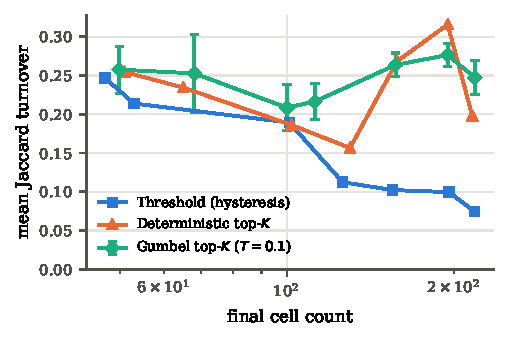
\includegraphics[width=\columnwidth]{figures/fig5_turnover.pdf}
\caption{Mean grid turnover against final cell count (second-order scheme, gradient indicator). Error bars: one standard deviation over 20 seeds (Gumbel top-$K$).}
\label{fig:turnover}
\end{figure}

\section{Discussion}
\label{sec:discussion}

The experiments rank the factors we varied by their effect on final error at matched cell count. Scheme order changes AMR error by a factor of 5.7--7.0. The indicator changes it by 1.13--1.85 with three levels, and refinement timing by 1.43--1.59 (Table~\ref{tab:timing}, A against C). The marking rule changes it by 3--30\%, and part of the larger figure reflects residual budget mismatch. In this setting the choice of marking rule is the least important of the four, and conclusions about it are only meaningful once the other three are fixed.

The separation between \emph{where} and \emph{how} explains several observations. With the first-order scheme, numerical diffusion on coarse cells is comparable to the physical viscosity, so the error is spread through the domain and resolution anywhere helps about equally (the first-order timing control). Placing refinement precisely cannot then pay off. With the second-order scheme, the error concentrates at the front, and both the timing control and the indicator ablation show that \emph{where} resolution is placed matters. The gradient indicator, however, ranks the smooth ramp highly because its slope is large, even though a piecewise-linear reconstruction represents a ramp almost exactly. That is a mismatch between the indicator and the error of the scheme it is guiding. The curvature indicator, whose leading term matches the error of a second-order reconstruction, removes most of this mismatch. The coarsening ablation shows that the mismatch cannot be repaired downstream: a stricter coarsening rule changes the budget and causes churn, but does not change which cells the indicator prefers.

The cost measure changes the conclusion. Per final cell, AMR looks favourable over a wider range of budgets than per unit of work, because a global time step charges every cell for the smallest one. Results reported only per degree of freedom therefore overstate the benefit of AMR for explicit schemes without subcycling. Conversely, part of the work penalty we report would disappear with subcycling \cite{berger1984,berger1989}.

Gumbel top-$K$ sampling did not improve accuracy or stability relative to deterministic top-$K$. At $\tau = 0.1$ the sampling occasionally selects low-ranked cells (Fig.~\ref{fig:meshes}), which neither helped nor clearly hurt. We did not find a regime in which smoothing the marking decision was beneficial.

\section{Limitations}
\label{sec:limitations}

The study uses a single one-dimensional problem, one viscosity, one initial condition, and one final time. A larger viscosity ($\nu = 0.03$) was tried as an alternative way to control numerical diffusion but was not used, because the front then becomes too wide to be a localized feature. The front is a resolved viscous layer; the results may differ for discontinuous solutions, systems of conservation laws, or two- and three-dimensional problems.

The solver has no local time stepping, which penalizes deep refinement (Section~\ref{sec:results}). D\"orfler marking \cite{dorfler1996} was not tested. Only one temperature ($\tau = 0.1$) was used for Gumbel top-$K$.

In the indicator ablation the gate is shared, so the results do not show how a fully curvature-based strategy (curvature-based gate and marking) would perform. Even with the shared gate rule, the regrid schedules after $t_g$ differ between arms, and a gate that stays open once triggered would remove this difference; we did not test that variant. The early-phase control uses fixed windows chosen from the known front location, and was run at a single budget.

The deterministic rules were run once per configuration; their variability under perturbed initial data was not measured. Budget matching is by final cell count and is approximate (for example, 112 against 126 cells at a target of 128). The shock window has a fixed half-width of 0.05. Reported uncertainties are standard deviations over Gumbel seeds and do not include other sources of variation.

\section{Conclusion}
\label{sec:conclusion}

We compared threshold, deterministic top-$K$, and Gumbel top-$K$ marking for AMR on the viscous Burgers' equation under matched budgets, and varied scheme order, refinement timing, coarsening threshold, and indicator in controlled experiments. The marking rule had the smallest effect of the factors studied, and temperature-scaled stochastic marking gave no consistent benefit in accuracy or mesh stability. Scheme order determined whether refinement could pay off at all. Refinement timing and the indicator determined where it paid off. The cost measure determined whether AMR appeared better than uniform refinement. With a second-order scheme and a curvature indicator, AMR was more accurate than uniform refinement at matched work at every budget tested with three refinement levels, a result that holds against actual uniform runs given at least as much work. Natural next steps are D\"orfler marking, a curvature-based gate, local time stepping, and problems with discontinuities and more than one space dimension.

\section*{Acknowledgment}

\textcolor{red}{[Author to edit or confirm.]} The numerical code, experiment scripts, and an initial draft of this manuscript were developed with the assistance of an AI system (Claude, Anthropic). The author reviewed the code, the results, and the text, and is responsible for all content.

\begin{thebibliography}{00}

\bibitem{berger1984}
M.~J. Berger and J.~Oliger, ``Adaptive mesh refinement for hyperbolic partial differential equations,'' \textit{J. Comput. Phys.}, vol.~53, no.~3, pp.~484--512, 1984.

\bibitem{berger1989}
M.~J. Berger and P.~Colella, ``Local adaptive mesh refinement for shock hydrodynamics,'' \textit{J. Comput. Phys.}, vol.~82, no.~1, pp.~64--84, 1989.

\bibitem{kool2019}
W.~Kool, H.~van Hoof, and M.~Welling, ``Stochastic beams and where to find them: The Gumbel-top-$k$ trick for sampling sequences without replacement,'' in \textit{Proc. 36th Int. Conf. Machine Learning (ICML)}, 2019, pp.~3499--3508.

\bibitem{babuska1978}
I.~Babu\v{s}ka and W.~C. Rheinboldt, ``Error estimates for adaptive finite element computations,'' \textit{SIAM J. Numer. Anal.}, vol.~15, no.~4, pp.~736--754, 1978.

\bibitem{dorfler1996}
W.~D\"orfler, ``A convergent adaptive algorithm for Poisson's equation,'' \textit{SIAM J. Numer. Anal.}, vol.~33, no.~3, pp.~1106--1124, 1996.

\bibitem{carstensen2014}
C.~Carstensen, M.~Feischl, M.~Page, and D.~Praetorius, ``Axioms of adaptivity,'' \textit{Comput. Math. Appl.}, vol.~67, no.~6, pp.~1195--1253, 2014.

\bibitem{lohner1987}
R.~L\"ohner, ``An adaptive finite element scheme for transient problems in CFD,'' \textit{Comput. Methods Appl. Mech. Eng.}, vol.~61, no.~3, pp.~323--338, 1987.

\bibitem{rusanov1962}
V.~V. Rusanov, ``The calculation of the interaction of non-stationary shock waves and obstacles,'' \textit{USSR Comput. Math. Math. Phys.}, vol.~1, no.~2, pp.~304--320, 1962.

\bibitem{vanleer1979}
B.~van Leer, ``Towards the ultimate conservative difference scheme. V. A second-order sequel to Godunov's method,'' \textit{J. Comput. Phys.}, vol.~32, no.~1, pp.~101--136, 1979.

\bibitem{gottlieb2001}
S.~Gottlieb, C.-W. Shu, and E.~Tadmor, ``Strong stability-preserving high-order time discretization methods,'' \textit{SIAM Rev.}, vol.~43, no.~1, pp.~89--112, 2001.

\bibitem{leveque2002}
R.~J. LeVeque, \textit{Finite Volume Methods for Hyperbolic Problems}. Cambridge, U.K.: Cambridge Univ. Press, 2002.

\bibitem{yang2023}
J.~Yang \textit{et~al.}, ``Reinforcement learning for adaptive mesh refinement,'' in \textit{Proc. 26th Int. Conf. Artificial Intelligence and Statistics (AISTATS)}, 2023.

\end{thebibliography}

\end{document}
